% 陈成：中文个人简历（带照片）
% 使用 XeLaTeX 编译：xelatex cheng-chen-resume-photo-zh.tex
\documentclass[UTF8,fontset=none,10pt,a4paper]{ctexart}

\usepackage[left=0.75cm,right=0.75cm,top=0.7cm,bottom=0.7cm]{geometry}
\usepackage{array}
\usepackage{enumitem}
\usepackage{fontawesome5}
\usepackage{fontspec}
\usepackage{graphicx}
\usepackage{hyperref}
\usepackage{needspace}
\usepackage{tabularx}
\usepackage{tikz}
\usepackage{xcolor}

\setmainfont{Times New Roman}
\setCJKmainfont{Songti SC}[AutoFakeBold=2]

\definecolor{accent}{HTML}{173F5F}
\definecolor{accenttwo}{HTML}{2D648C}
\definecolor{sidebar}{HTML}{EEF3F7}
\definecolor{text}{HTML}{27333D}
\definecolor{muted}{HTML}{687782}
\definecolor{line}{HTML}{CBD6DE}

\hypersetup{
  colorlinks=true,
  urlcolor=accent,
  linkcolor=accent,
  pdfauthor={Cheng Chen},
  pdftitle={陈成个人简历}
}

\pagestyle{empty}
\setlength{\parindent}{0pt}
\setlength{\parskip}{0pt}
\setlength{\tabcolsep}{0pt}
\color{text}
\fontsize{9.5}{11.4}\selectfont

\setlist[itemize]{
  leftmargin=1.15em,
  label=\textcolor{accenttwo}{\small\textbullet},
  itemsep=0.5pt,
  topsep=1.5pt,
  parsep=0pt,
  partopsep=0pt
}

\newcommand{\leftsection}[1]{%
  \vspace{9pt}%
  {\normalsize\bfseries\color{accent}#1}\par
  \vspace{-2pt}\textcolor{line}{\rule{\linewidth}{0.6pt}}\vspace{4pt}%
}

\newcommand{\rightsection}[1]{%
  \needspace{4\baselineskip}%
  \vspace{6pt}%
  {\Large\bfseries\color{accent}#1}\par
  \vspace{-2pt}\textcolor{line}{\rule{\linewidth}{0.7pt}}\vspace{3pt}%
}

\newcommand{\entry}[4]{%
  \needspace{6\baselineskip}%
  \begin{tabularx}{\linewidth}{@{}>{\raggedright\arraybackslash}X>{\raggedleft\arraybackslash}p{2.25cm}@{}}
    {\bfseries\color{accent}#1} & {\small\color{muted}#3}
  \end{tabularx}\par
  {\small\color{muted}#2}\par
  \vspace{-1pt}
  \begin{itemize}#4\end{itemize}
}

\newcommand{\contactline}[2]{%
  \begin{tabularx}{\linewidth}{@{}p{0.52cm}X@{}}
    \textcolor{accent}{#1} & #2
  \end{tabularx}\vspace{2pt}%
}

\begin{document}

\begin{tikzpicture}[remember picture,overlay]
  \fill[sidebar] (current page.north west)
    rectangle ([xshift=6.25cm]current page.south west);
\end{tikzpicture}

\noindent
\begin{minipage}[t][0.965\textheight][t]{5.05cm}
  \vspace{0pt}
  \begin{center}
    \setlength{\fboxsep}{2.5pt}
    \setlength{\fboxrule}{0.7pt}
    \fcolorbox{white}{white}{%
      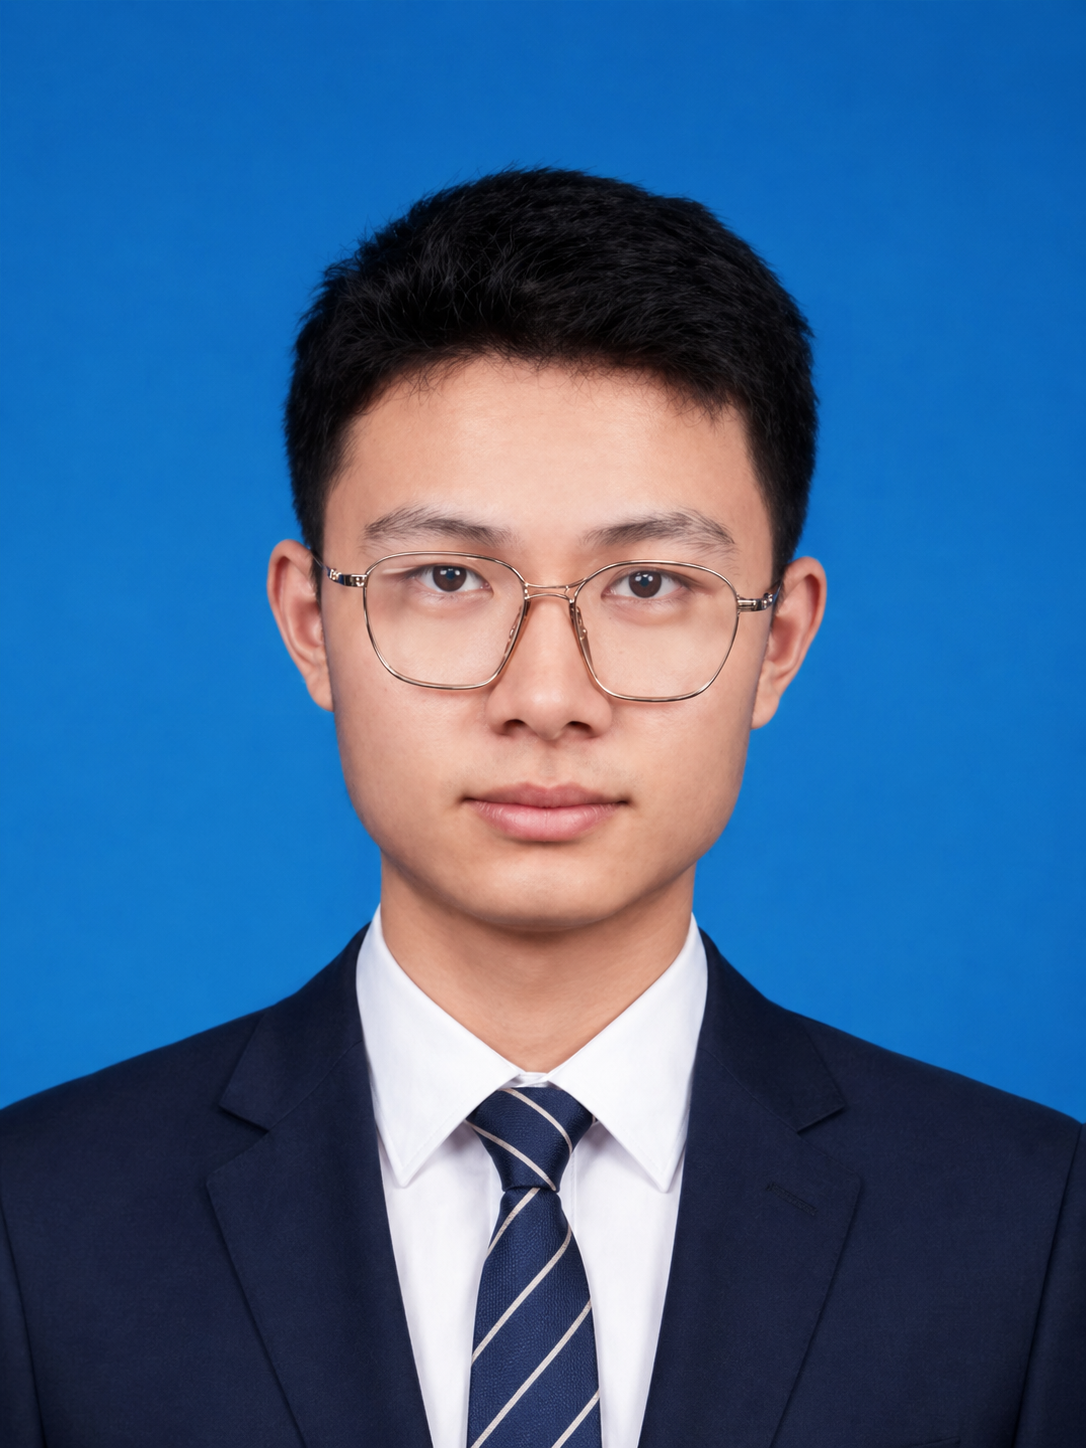
\includegraphics[width=3.05cm,height=4.06cm,keepaspectratio]{me.png}%
    }
  \end{center}

  \leftsection{联系方式}
  \contactline{\faEnvelope[regular]}{\href{mailto:2351445@tongji.edu.cn}{2351445@tongji.edu.cn}}
  \contactline{\faPhone}{(+86) 13587919792}
  \contactline{\faGlobe}{\href{https://ceasonen.github.io}{ceasonen.github.io}}
  \contactline{\faGithub}{\href{https://github.com/ceasonen}{github.com/ceasonen}}
  \contactline{\faGraduationCap}{\href{https://scholar.google.com/citations?user=X92zQ68AAAAJ}{Google Scholar}}
  \contactline{\faMapMarker}{上海，中国}

  \leftsection{教育背景}
  {\bfseries 中国科学院自动化研究所}\par
  博士生（拟入学），导师：黄凯奇老师\par
  2026.09 至今\par
  \vspace{3pt}
  {\bfseries 同济大学}\par
  通信工程，本科在读\par
  2023.09 至 2027.06（预计）\par
  \vspace{3pt}
  专业排名：\textbf{3/85}

  \leftsection{研究兴趣}
  \begin{itemize}
    \item 多模态学习
    \item 高效人工智能
    \item 推理与可靠人工智能
    \item 大语言模型
    \item 多模态大模型
    \item 具身智能与强化学习
  \end{itemize}

  \leftsection{专业能力}
  \textbf{编程：}Python，C/C++，Verilog\par
  \textbf{框架：}PyTorch\par
  \textbf{工具：}Git，Linux，\LaTeX\par
  \textbf{辅助开发：}OpenAI Codex，Claude Code\par
  \textbf{基础：}机器学习、算法、线性代数、概率论、优化方法、信号处理

  \vfill
\end{minipage}
\hspace{0.66cm}
\begin{minipage}[t][0.965\textheight][t]{12.95cm}
  \vspace{0pt}
  {\fontsize{29}{32}\selectfont\bfseries\color{accent}陈成}\par
  \vspace{2pt}
  {\large\color{muted}中国科学院自动化研究所 · 博士生（拟入学）}\par
  \vspace{7pt}
  已获中国科学院自动化研究所博士生录取，拟在黄凯奇老师指导下继续围绕神经算子可靠性、知识蒸馏与多模态学习开展研究，关注计算高效、具备推理能力并适应真实应用条件的人工智能方法。

  \rightsection{科研经历}

  \entry{神经算子可靠性评估}{神经信息处理系统大会（NeurIPS，CCF A 类） · 2026 投稿 · 第一作者 · 审稿中}{2024 至 2026}{
    \item 研究神经算子的部署可靠性，解决传统不确定性方法依赖重复推理、削弱快速场预测效率优势的问题。
    \item 提出分配不确定性分解方法，从预测路径的分配熵构造单次前向风险分数，无需后验采样或额外不确定性分支。
    \item 在电磁散射任务上，将斯皮尔曼相关系数由 \textbf{0.61} 提升至 \textbf{0.67}，失效检测曲线下面积由 \textbf{0.78} 提升至 \textbf{0.82}；选择性升级后分别达到 \textbf{0.72} 和 \textbf{0.85}。
  }

  \entry{OV-OrthKD}{ACM 国际多媒体会议 2026（ACM MM，CCF A 类） · 共同一作 · 已录用}{2025 至 2026}{
    \item 研究开放词汇音视频事件定位中的模态可靠性不对称，避免画外音、时延和噪声干扰时间边界学习。
    \item 强视觉教师负责决策相关特征，弱音频教师被限制在辅助正交子空间，文本原型用于开放词汇迁移。
    \item 在 OV-AVEBench 上取得 \textbf{0.816} 分段平均精度，整体与未见类别在阈值 0.5 下的 F1 分数较官方微调基线提高 \textbf{2.7} 和 \textbf{3.4} 个百分点。
  }

  \entry{OrthKD}{国际人工智能联合会议 2026（IJCAI，CCF A 类） · 共同一作 · 已录用}{2024 至 2026}{
    \item 研究糖尿病视网膜病变筛查中的异构多教师蒸馏，处理弱教师分类得分损害学生模型的问题。
    \item 由强教师提供完整监督，仅提取弱教师的互补特征，并以正交约束减少教师特定表征之间的冗余。
    \item 在 \textbf{132{,}049} 张眼底图像上，\textbf{540 万}参数的 MobileNetV3 在 EyePACS 上达到 \textbf{0.885} 二次加权 Kappa，Messidor-2 零样本结果由 \textbf{0.507} 提升至 \textbf{0.728}。
  }

  \rightsection{竞赛与荣誉}
  \begin{itemize}
    \item \textbf{全国一等奖}，中国机器人及人工智能大赛，队长，2026
    \item \textbf{全国二等奖}，全球校园人工智能算法精英大赛，队长，2025
    \item \textbf{全国三等奖}，全国大学生嵌入式芯片与系统设计竞赛，队长，2025
    \item 同济大学本科优秀学生奖学金二等奖，2023/2024、2024/2025
  \end{itemize}
\end{minipage}

\end{document}
